


\label{sec:evaluation}

This section answers the following questions:
\begin{itemize}
\item
  How effective is \Predator{} at detecting and predicting false sharing?

\item
  What is \Predator{}'s overhead, in terms of execution time and memory ?

\item
  How sensitive is \Predator{} to different sampling rates?
 
\end{itemize}

\paragraph{Experimental Platform.} All evaluations are performed on a quiescent Intel Core 2 dual-processor system equipped with 
16GB RAM. Each processor is a 4-core 64-bit Intel Xeon running at 2.33 GHz, with a 4MB shared L2 cache and 32KB private L1 cache. The underlying operating system is an unmodified CentOS 5.5, running with Linux kernel version 2.6.18-194.17.1.el5. The glibc version is 2.5. 

\paragraph{Evaluated Applications.}
This paper evaluates two popular benchmark suites,
Phoenix (with large input) ~\cite{phoenix-hpca} and PARSEC (with simlarge input) ~\cite{parsec}. Even with unmodified LLVM-3.2, Facesim cannot be compiled successfully (having complaints on an undefined template) and Canneal aborts unexpectedly. Thus, these two benchmarks are excluded.
We also evaluate \Predator{} on six real applications, including MySQL, Boost, Memcached, aget, pbzip2 and pfscan.



\subsection{Detection and Prediction Effectiveness}
\label{sec:effective}

\begin{figure*}[htb]
{\centering
\tiny
\subfigure{\lstinputlisting[numbers=none,frame=none,boxpos=t]{predator/figure/linearregression.report}}
\caption{An example report by \Predator{} indicating false sharing in the linear\_regression benchmark.
\label{fig:lrreport}}
}
\end{figure*}

For every false sharing problem, \Predator{} reports source code information and detailed memory access information in order to help users fix those problems. Figure~\ref{fig:lrreport} shows an example for the linear\_regression benchmark. This report shows that the heap object starting with $0x40000038$ potentially causes a large number of cache invalidations. The call stack of allocation is provided to help locate culprits. In addition, \Predator{} also reports word-level access information of this object, which helps to identify where and how false sharing occurs. From that, we can know that it is a latent false sharing problem predicted by \Predator{}, since different threads are accessing different cache lines. 

\subsubsection{Benchmarks}
\label{sec:benchmarks}

\begin{table*}[!t]
{\centering\begin{tabular}{l|r|r|r|r|r}\hline
{\bf \small Benchmark} & {\bf \small Source Code} & {\bf \small New} & {\bf \small Without Prediction} &{\bf \small With Prediction} & {\bf \small Improvement} \\
\hline
\small \textbf{histogram} & {\small histogram-pthread.c:213} & \cmark{} &\cmark{} & \cmark{} & 46.22\%\\
\small \textbf{linear\_regression} & {\small linear\_regression-pthread.c:133} & & & \cmark{} & 1206.93\% \\
\small \textbf{reverse\_index} & {\small reverseindex-pthread.c:511} & & \cmark{} & \cmark{} & 0.09\%\\
\small \textbf{word\_count} & {\small word\_count-pthread.c:136} & & \cmark{} & \cmark{} & 0.14\%\\
\hline
\small \textbf{streamcluster} & {\small streamcluster.cpp:985} &  & \cmark{} & \cmark{} &7.52\% \\
\small \textbf{streamcluster} & {\small streamcluster.cpp:1907} & \cmark{} & \cmark{} & \cmark{} & 4.77\%\\
\hline
\end{tabular}
\caption{False sharing problems in the Phoenix and PARSEC benchmark suites. \label{table:detection}}
}
\end{table*}

Table~\ref{table:detection} provides detection results of two benchmark suites, Phoenix and PARSEC
The first column lists those programs with false sharing problems.  The second column shows precisely where the problem is. Because all discovered false sharing occurs inside heap objects, we show callsite source code information here.  The third column, ``New'', marks whether this false sharing was newly discovered by \Predator{}.  A checkmark in the following two columns indicates whether the false sharing was identified without
prediction and/or with prediction.  The final column, ``Improvement'', shows the performance improvement after fixing false sharing.
%The number is based on the average runtime of $10$ runs. 

As shown in the table, \Predator{} reveals two unknown false sharing problems. It is the first tool to detect the false sharing problems in histogram and in line $1908$ of streamcluster. 
In histogram, multiple threads simultaneously modify different locations of the same heap object, thread\_arg\_t. 
Padding this data structure fixes the false sharing problem and improves the performance by around 46\%. In streamcluster, multiple threads are simultaneously accessing and updating the same \texttt{bool} array, switch\_membership. Simply changing all elements of this array to a long type reduces the false sharing and improves the performance by about 4.7\%.

%, although it is not a complete fix of false sharing. 
%None of these two false sharing problems has been reported by previous tools.
Other false sharing problems were discovered by previous work~\cite{sheriff}. We do not see significant performance improvement for reverse\_index and word\_count benchmarks. They are reported here because the number of cache invalidations in these two programs reaches our predefined threshold.
Making the reporting threshold higher can avoid the report of those insignificant false sharing problems.
It is worth noting that these two benchmarks definitely have false sharing problems,
which can be confirmed by word-level information generated by \Predator{}. 

The streamcluster benchmark has another false sharing problem at line $985$. Different threads change the work\_mem object simultaneously. Authors of streamclsuter have already realized this problem and provide a CACHE\_LINE macro. Unfortunately, the default value of this macro is set to $32$ bytes, which is different from the actual cache line size of the experimental machine. By setting it to $64$ bytes instead, it achieves  performance improvement of about 7.5\%.

linear\_regression has a severe false sharing problem. Fixing it improves the performance by more than $12\times$. In this benchmark, different threads update their thread-specific locations inside the tid\_args object in a tight loop. According to the observation of Nanavati et al., this false sharing problem occurs when using clang and disappears when using gcc with the -O2 and -O3 optimization level~\cite{OSdetection}. But we observed a different result when using the clang-3.2 compiler and our custom memory allocator: the false sharing problem does not occur at all because the offset of the starting address of the potentially falsely-shared object and the start of cache line is 56 bytes (see Figure~\ref{fig:perfsensitive}). With prediction mechanism, \Predator{} detects this latent false sharing problem, exemplifying the necessity of a predictive detection tool. 

\subsubsection{Real Applications}
To verify \Predator{}'s practicality, we further evaluate several widely-used real applications, whereas no previous work has done this. These real applications include a server application (MySQL~\cite{mysql}),
a standard C++ library (Boost~\cite{libfalsesharing}),
a distributed memory object caching system (Memcached), a network retriever (aget),
a parallel bzip2 file compressor (pbzip2), and a parallel file scanner (pfscan).

MySQL-5.5.32 and boost-1.49.0 are known to have false sharing problems. Other applications (memcached-1.4.15, aget-0.4.1 and pbzip2-1.1.6) do not have known false sharing problems.

The false sharing of MySQL has caused a significant scalability problem and was very difficult to identify.
According to the architect of MySQL, Mikael Ronstrom, ``we had gathered specialists on InnoDB..., participants from MySQL support... and a number of generic specialists on 
computer performance...'', ``[we] were able to improve MySQL performance by 6$\times$ with those scalability fixes''~\cite{mysql}. 
The false sharing inside Boost is caused by the usage of a  spinlock pool. Different threads may utilize different spinlocks located in the same cache line in this case. Fixing it brings a 40\% performance improvement.
\Predator{} is able to pinpoint false sharing locations in both MySQL and the Boost library. 
For the other four applications, \Predator{} does not find severe false sharing problems.

\subsubsection{Prediction Effectiveness}
\label{sec:predicteval}
In this section, we verify whether prediction can always  reveal un-observed false sharing problems.

The linear\_regression benchmark is selected here because of the following two reasons: (1) The false sharing problem of this benchmark cannot be detected without prediction; (2) False sharing severely degrades performance when it actually occurs. Hence, it is a serious problem that should always be detected. 

\begin{figure}[!t]
{\centering
\subfigure{\lstinputlisting[numbers=none,frame=none,boxpos=t]{predator/figure/linearregression.psedocode}}
\caption{The false sharing problem inside the linear\_regression benchmark: multiple threads simultaneously update their entries in lreg\_args.
\label{fig:linearregression}}
}
\end{figure}

Figure~\ref{fig:linearregression} shows the data structure and the source code exercising appropriate false sharing. The size of this data structure, lreg\_args, is $64$ bytes 
when the program is compiled to a $64$-bit binary. For this benchmark, the main thread allocates an array, containing as many elements as the number of underlying hardware cores. Each element is a lreg\_args type with $64$ bytes. This array is then passed to different threads (lreg\_thread function) so that each thread only updates its thread-dependent area. False sharing occurs if two threads happen to update data in the same cache line. 

Figure~\ref{fig:perfsensitive} shows how sensitive the performance is to different starting addresses of a falsely-shared object. When the offset is $0$ or $56$ bytes, this benchmark achieves its optimal performance and has no false sharing. When the offset is $24$ bytes, the benchmark runs around $15$ times slower than its optimal performance because of the false sharing problem.

Our evaluation shows that \Predator{} can always detect the false sharing problem with prediction enabled, demonstrating its effectiveness.

\subsection{Performance Overhead}
\label{sec:perfoverhead}

\begin{figure*}[!t]
\centering
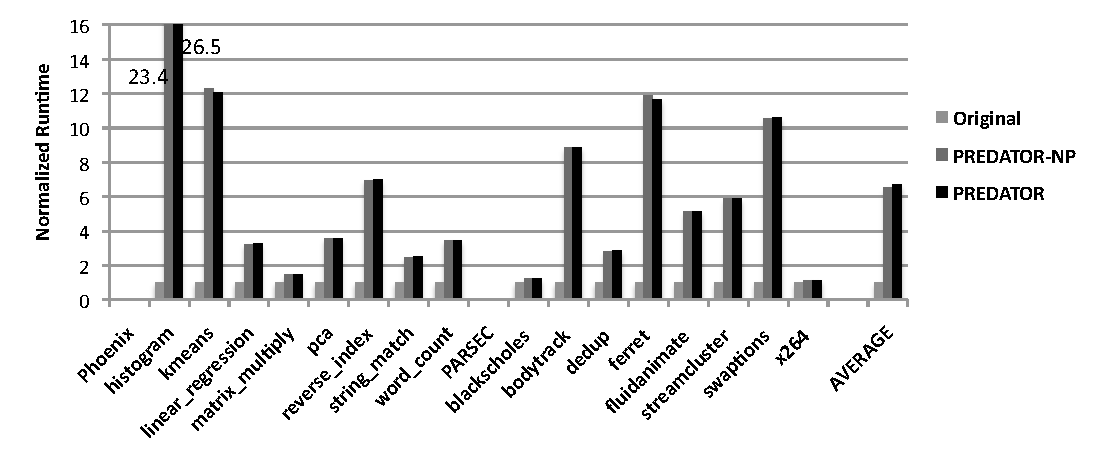
\includegraphics[width=6in]{predator/figure/perf}
\caption{
Performance overhead of \Predator{} with and without prediction(PREDATOR-NP).
\label{fig:perf}}
\end{figure*}

To avoid the effect caused by extreme outliers, all performance data shown in Figure~\ref{fig:perf} is based on the average of $10$ runs, excluding the maximum and minimum values. 

For $16$ benchmarks from the Phoenix and PARSEC benchmark suites and six real applications, \Predator{} imposes $5.4\times$ performance overhead. There is no noticeable difference on performance whether the prediction mechanism is enabled or not. 
 
Among these programs, five of them, histogram, kmeans, bodytrack, ferret, and swaptions, have more than $8\times$ performance overhead. The histogram benchmark runs more than $26\times$ slower than original executions with \pthreads{} library, because tracking detailed access on cache lines with false sharing exacerbates the false sharing effect (see more discussion in Section~\ref{sec:sample}).  For bodytrack and ferret, although there is no false sharing, \Predator{} detects a large amount of cache lines with writes larger than {\it Tracking-Threshold}. Thus, tracking those accessing details for those cache lines imposes significant performance overhead. Currently, we cannot identify the reasons why kmeans runs very slowly on \Predator{}.
   
\Predator{} imposes a small performance overhead for IO-bound applications, such as matrix\_multiply, blackscholes, x264, aget, Memcached, pbzip2, and pfscan, since \Predator{} does not add any performance overhead for IO operations.  

\subsection{Memory Overhead}
\label{sec:memoverhead}
We only evaluate the physical memory overhead of \Predator{}, instead of the virtual memory overhead, because \Predator{} allocates four gigabytes virtual memory for its custom memory allocator. Proportional set size (PSS) in \texttt{/proc/self/smaps} reflects the physical memory increase on the existing system of running an application~\cite{memusage}. Thus, we periodically collect this data and use the sum of different memory mappings as the total physical memory usage of running an application. We present the maximum value of physical memory usage in Figure~\ref{fig:memusage}. 

\Predator{} imposes less than 50\% memory overhead for 17 out of 22 applications.  For swaptions and aget, \Predator{} introduces more memory overhead because the original memory footprints of them are very small, only $3$ kilobytes. Adding the code of detection, prediction and reporting contributes to a large ratio of memory overhead. We are not clear why MySQL consumes much more memory than others. Although the average memory usage of all applications is over $2\times$, the total memory usage overhead is only about $40\%$ on \Predator{}. 


\subsection{Sensitivity to Different Sampling Rates}
\label{sec:sensitivity}
In Section~\ref{sec:sample}, we discuss that \Predator{} utilizes the sampling mechanism to reduce the tracking overhead. Running an application with different sampling rates does not affect its memory usage. Thus, we only evaluate the effect of different sampling rates on performance and effectiveness. 

The default sampling rate used by \Predator{} is 1\%. In this section, we also evaluate two other sampling rates, 0.1\% and 10\%. The performance results under the three different sample rates are shown in Figure~\ref{predator/figure:sample}. \Predator{} introduces less performance overhead under a lower sampling rate, which meets our expectation. Concerning effectiveness, even using the 0.1\% sampling rate, \Predator{} can still detect all false sharing problems, but with a lower number of cache invalidations. Thus, different sampling rates do not affect the detection effectiveness.
 
\begin{figure*}[!t]
\centering
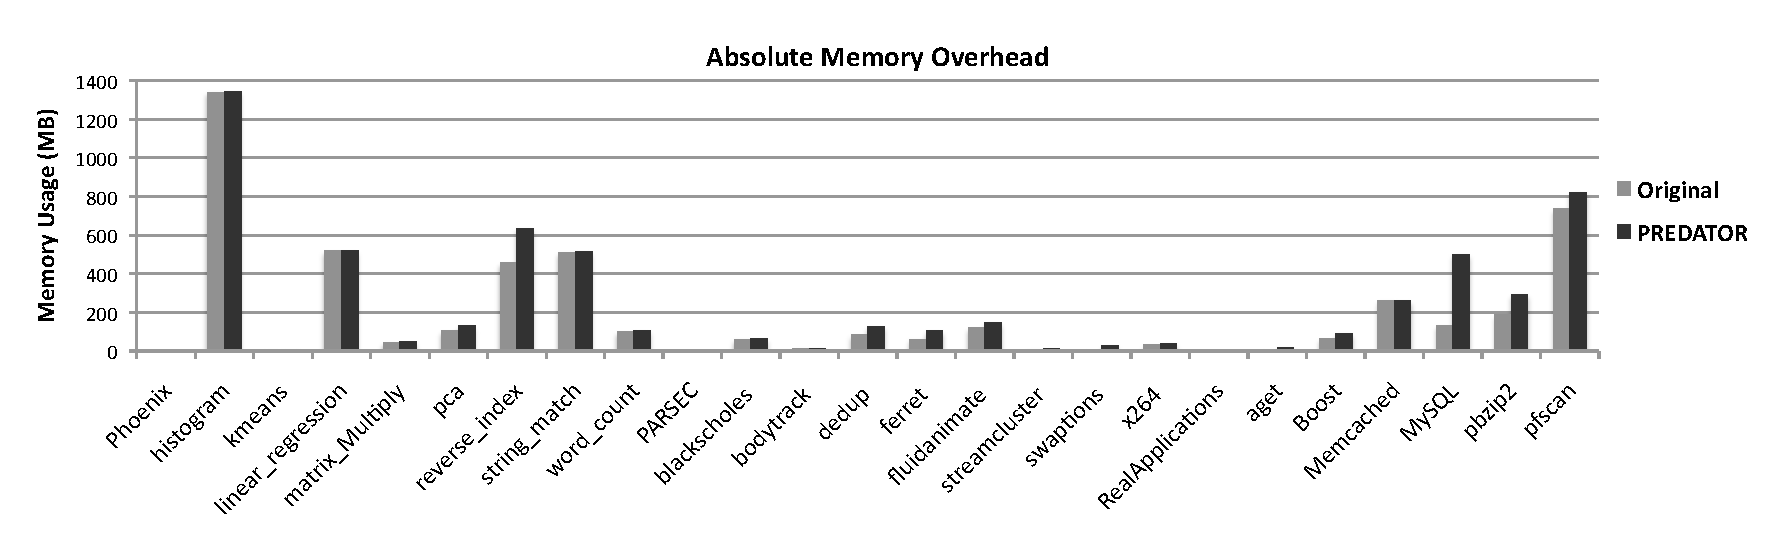
\includegraphics[width=6in]{predator/figure/absolutememory}
\caption{Absolute physical memory usage overhead with \Predator{}.}
\label{fig:absolutememusage}
\end{figure*}

\begin{figure*}[!t]
\centering
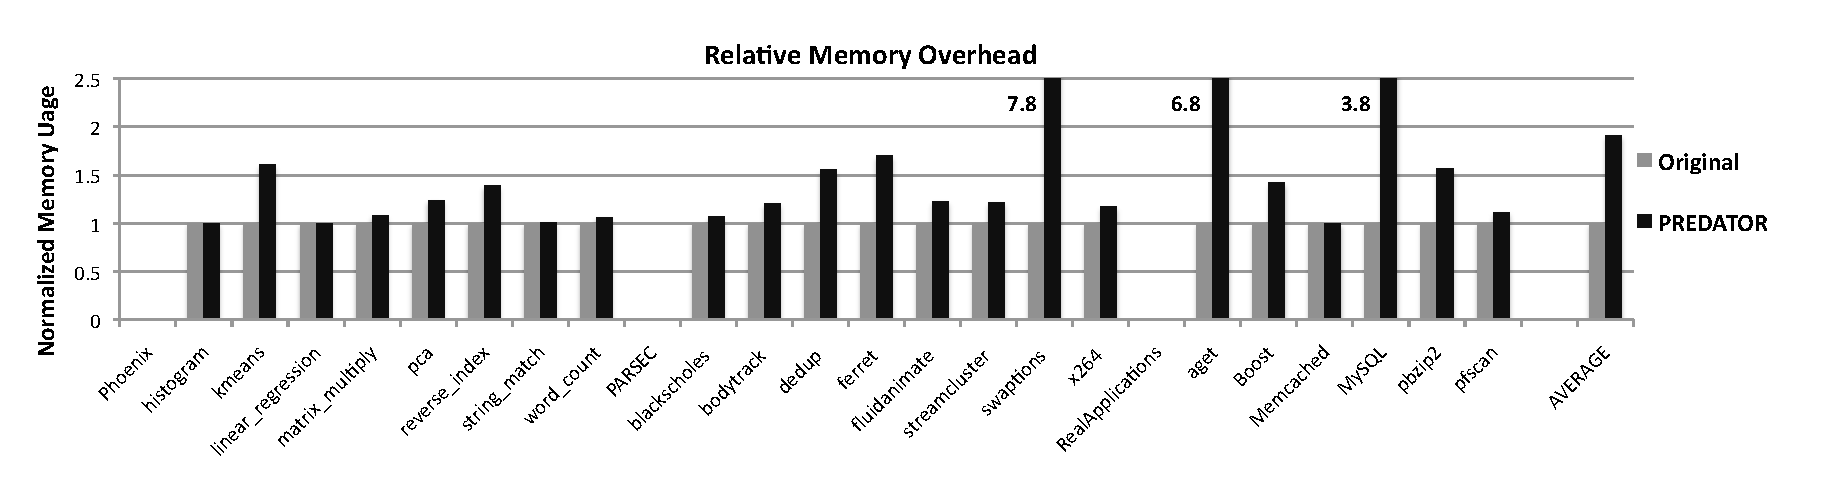
\includegraphics[width=6in]{predator/figure/memusage}
\caption{Relative physical memory usage overhead with \Predator{}.}
\label{fig:memusage}
\end{figure*}

